\section{Data Reports}
\label{sec:datareports-webapp}

The second web application, called \textit{Data Reports}, aims to retrieve, through preset \ac{SPARQL} queries, the \acl{LOD} uploaded in the phase described in Chapter \ref{chp:rdf-builder}, process them and display them in an understandable way by means of tables, graphs and maps. In fact, the basic idea is to create an online journal where different data are displayed and commented on for each article and grouped by semantic area.

As for the CKAN portal described in Section \ref{sec:ckan-webapp}, the application is containerized in a Docker image to simplify its installation and adoption. The application is open source, and it is available on GitHub at \url{https://github.com/luca-martinelli-09/ontoim-webapp}. A snapshot of the web application's home page configured for the Comune di Sona is shown in Figure \ref{fig:data-reports-home}.

\begin{figure}[!ht]
  \centering
  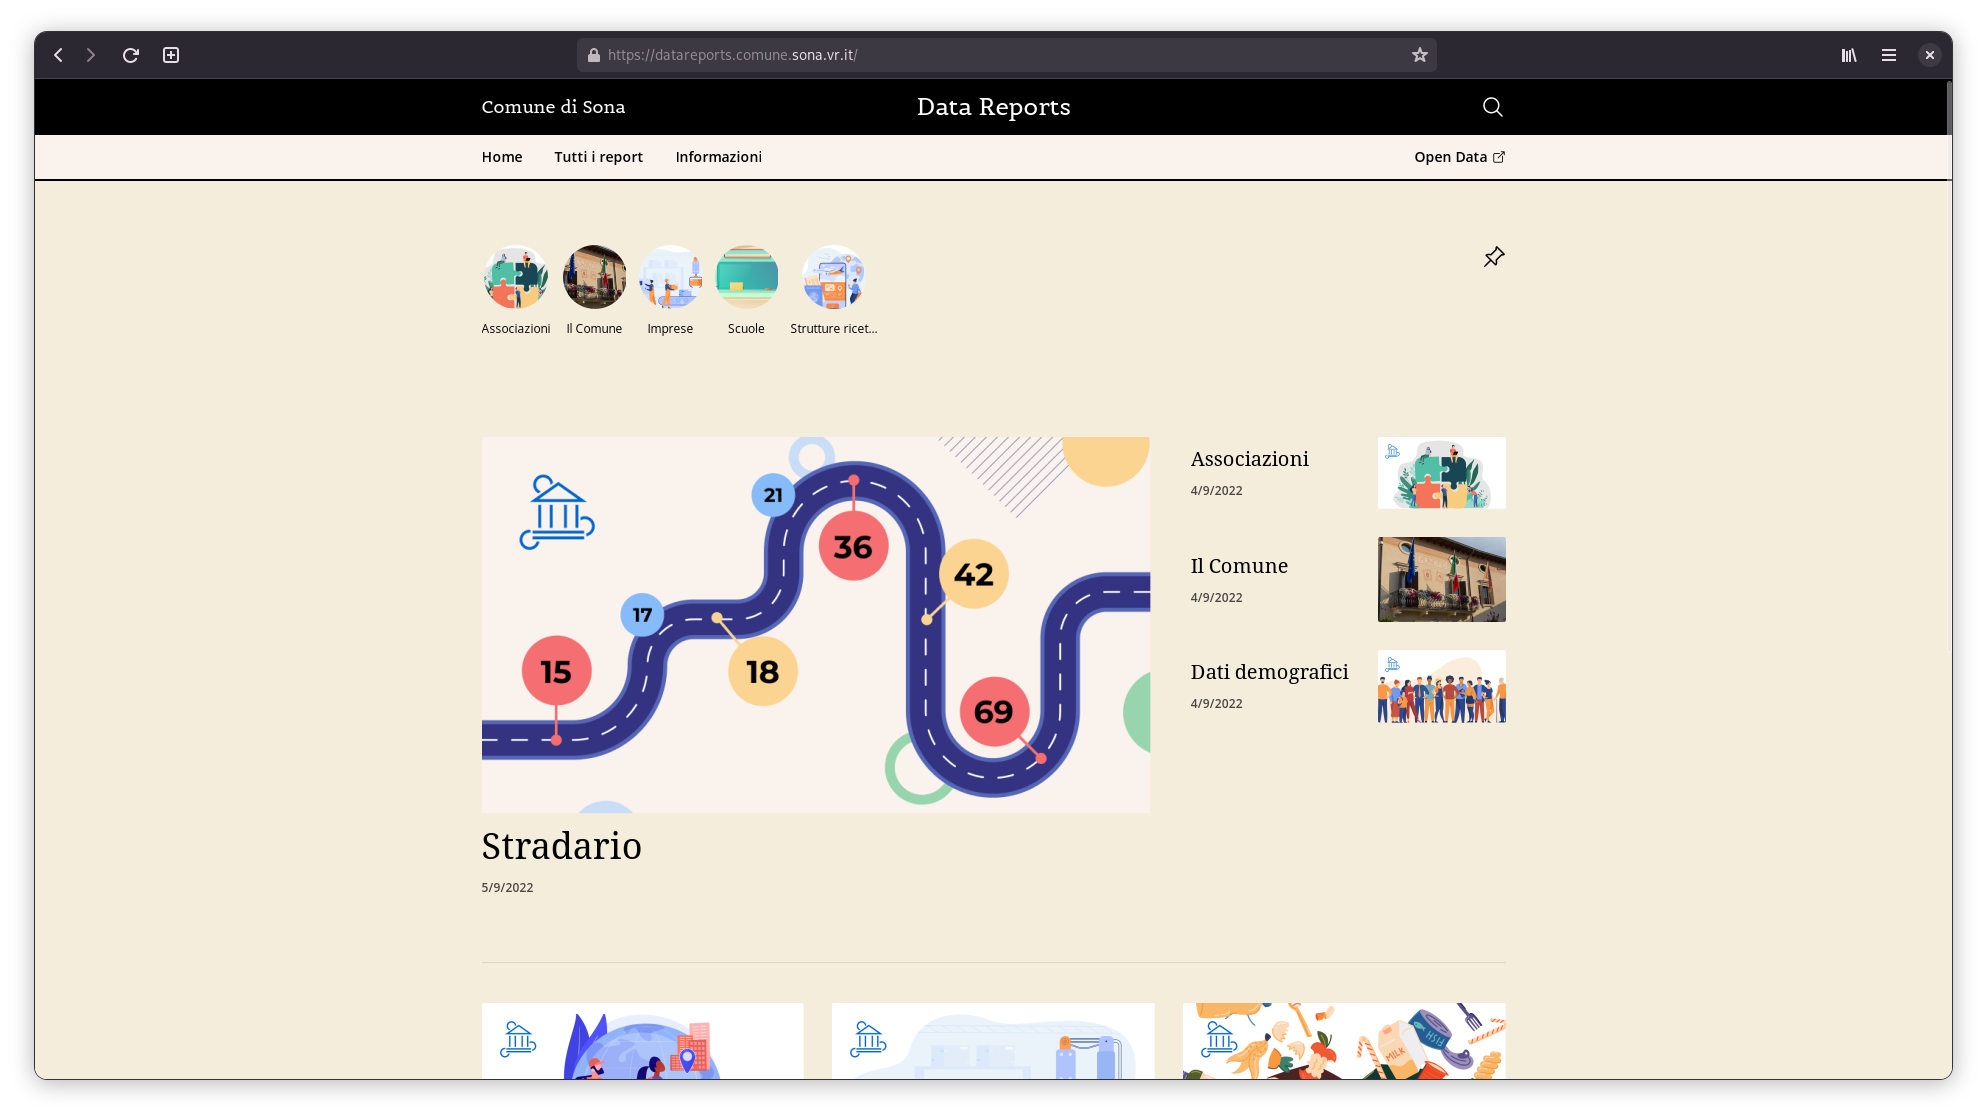
\includegraphics[width=\columnwidth]{images/datareports/datareports-home}
  \caption{A snapshot of the Data Reports home page.}
  \label{fig:data-reports-home}
\end{figure}

\textit{Data Reports} was developed using Svelte,\footnote{\url{https://svelte.dev/}} and SvelteKit,\footnote{\url{https://kit.svelte.dev/}} a modern JavaScript framework for building fast and \acs{SEO} friendly web applications. Unlike other frameworks such as Vue\footnote{\url{https://vuejs.org/}} or React,\footnote{\url{https://reactjs.org/}} in fact, Svelte produces all the files necessary for the site to function at the \textit{compile step}. In addition, Svelte, being a JavaScript framework, can be integrated with numerous ready-made packages available on the npm\footnote{\url{https://www.npmjs.com/}} package manager. Svelte also supports the creation of components, which are small pieces of code that can be imported and reused on multiple pages. Some of these packages are called \textit{preprocessors}, which Svelte uses to compile code and produce web pages. Some of these, for example, create \acs{SEO} friendly links, others compact \acs{HTML} code, and others generate \acs{CSS}. The full documentation of all the features of Svelte is available at \url{https://kit.svelte.dev/docs/introduction}.

\textit{Data Reports} uses several packages and preprocessors, the most relevant of which are:

\begin{description}
  \item[TailwindCSS and PostCSS] They provide a modern \acs{CSS} framework that aims to speed up website development, easy to customize, adaptable, and using \acs{CSS} best practices;
  \item[MDsveX] It is a preprocessor for Svelte that process Markdown files and convert them to \acs{HTML}. It also supports Svelte components, scripts, \acs{HTML} tags, and YAML headers, which let add information to the pages, like the publication date or the title;
  \item[Apache ECharts] It is an open source library for data visualization. It allows you to easily create interactive charts, maps, and more;
  \item[Leaflet] It is the leading open source library for creating interactive maps using OpenStreetMap\footnote{\url{https://www.openstreetmap.org/}}.
\end{description}

Each page/report is therefore a Markdown file that contains a YAML header which specifies the title of the report, the publishing date, a \ac{URL} for the thumbnail image, and some tags used for classification. Then, the text (e.g. description of the data, some comments on them), is written in Markdown in the body of the page. Code \ref{code:datareports-associations} shows the Markdown page that displays the list of associations registered in the Comune di Sona, the map where these associations are located, and a pie chart on the number of associations by type. Figure \ref{fig:datareports-examples} shows the pages related to demographic statistics and citizenship of foreign citizens. To increment the readability and reusability of the code, each part of the page involved in retrieving and displaying data was converted into a Svelte component that could be embedded.

\lstset{literate={è}{{\`e}}1}
\begin{lstlisting}[language=HTML,caption={"Associazioni" report page in Markdown.},label=code:datareports-associations]
---
title: Associazioni
date: 2022-09-04
fixed: true
thumb: /reports/thumb-associations.png
keywords:
  - associazioni
---

<script>
  import TabellaAssociazioni from "../data/associazioni/TabellaAssociazioni.svelte";
  import MappaAssociazioni from "../data/associazioni/MappaAssociazioni.svelte";
  import TipologiaAssociazioni from "../data/associazioni/TipologiaAssociazioni.svelte";
</script>

In questa sezione è possibile consultare l'albo delle associazioni del Comune di Sona, con le relative informazioni.
<TabellaAssociazioni />

Di seguito la mappa delle associazioni
<MappaAssociazioni />

## Tipologia di associazioni
<TipologiaAssociazioni />
\end{lstlisting}

\begin{figure}[!ht]
  \begin{subfigure}{.5\columnwidth}
    \centering
    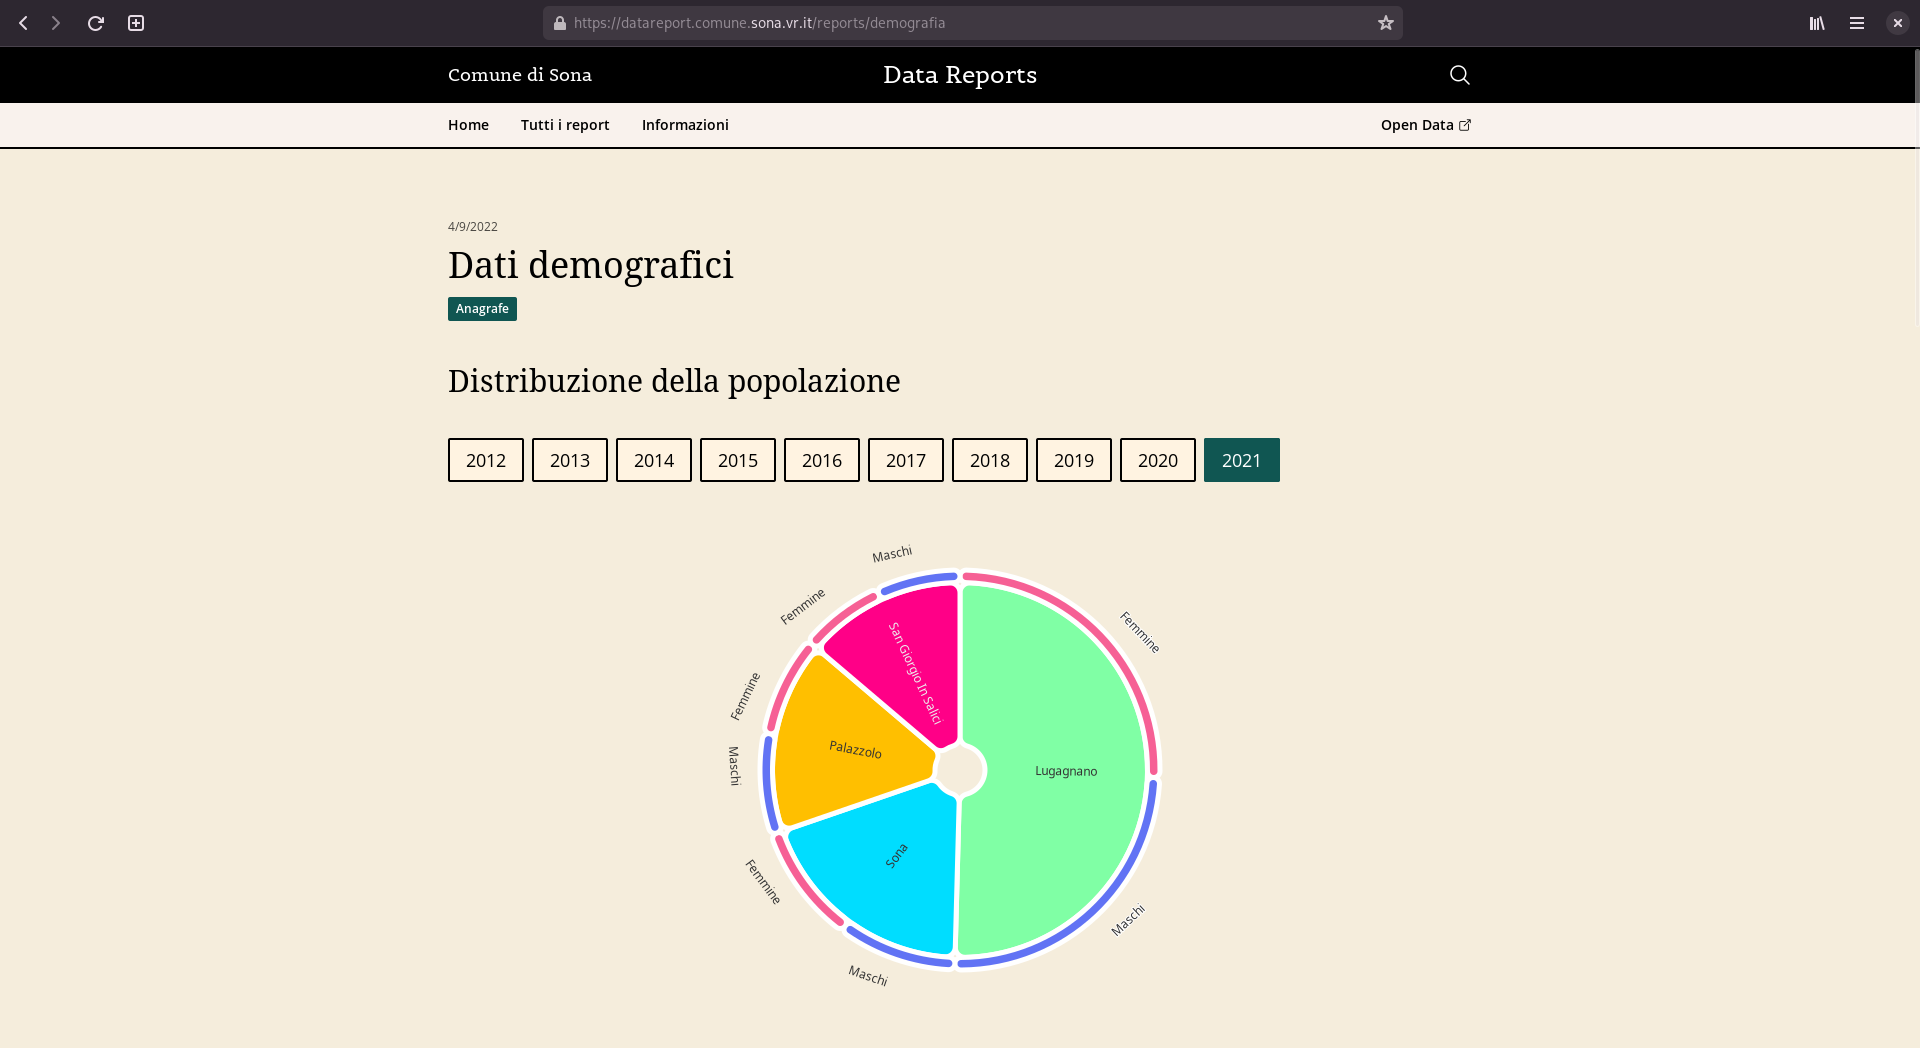
\includegraphics[width=\columnwidth]{images/datareports/datareports-demography}
    \subcaption{"Dati demografici" report.}
    \label{fig:datareports-demography}
  \end{subfigure}%
  \begin{subfigure}{.5\columnwidth}
    \centering
    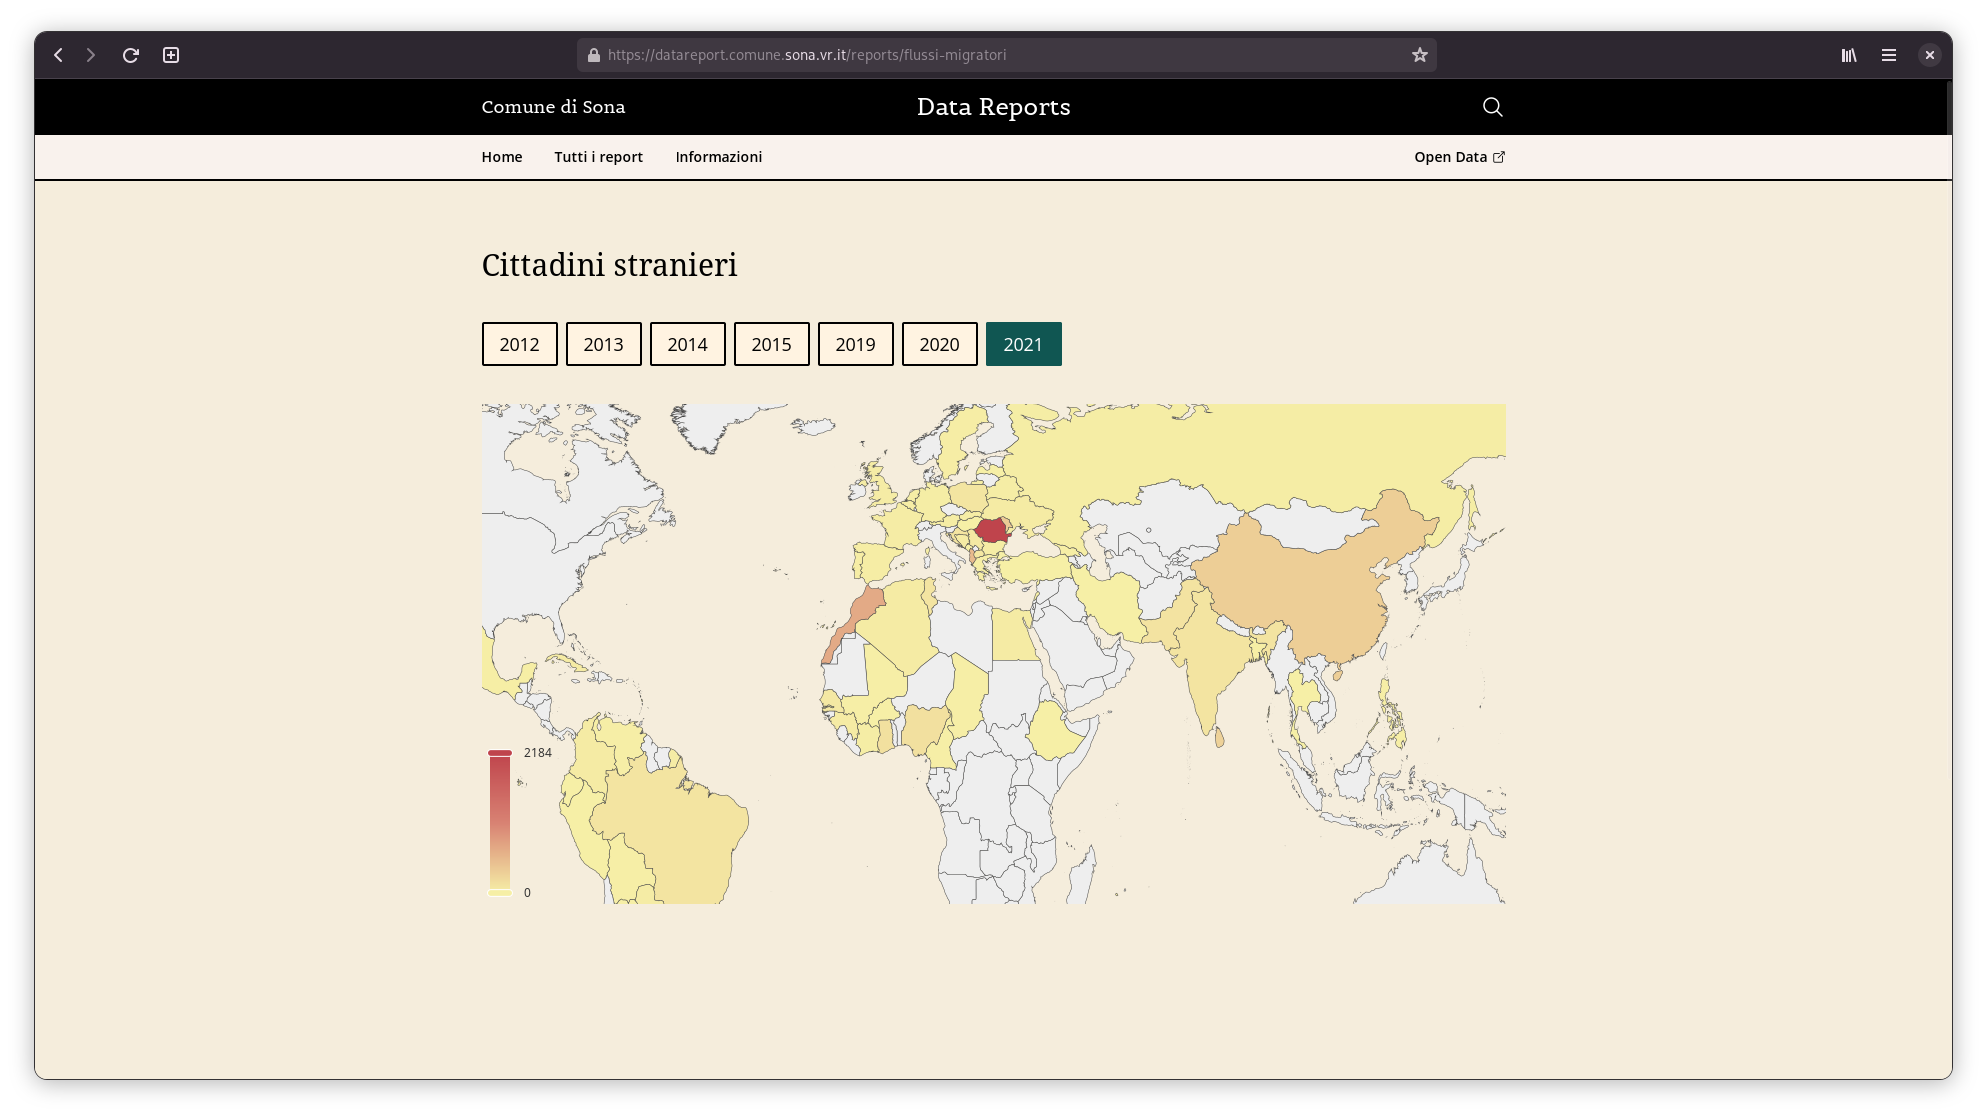
\includegraphics[width=\columnwidth]{images/datareports/datareports-citizenship}
    \subcaption{"Flussi migratori e cittadinanza" report.}
    \label{fig:datareports-citizenship}
  \end{subfigure}
  \caption{Snapshots for different Data Reports's pages.}
  \label{fig:datareports-examples}
\end{figure}

Each of these components is responsible for running a \ac{SPARQL} query to the endpoint, and processing the result, in \ac{JSON} format, to constitute the configuration that generates the charts, tables and maps. The function that execute the \ac{SPARQL} query, called \verb#querySPARQL#, is common to all components, so it was defined in a \verb#utils# script that is imported. Code \ref{code:query-sparql} shows the \verb#querySPARQL# function.

\begin{lstlisting}[language=Java,caption={The querySPARQL function.},label=code:query-sparql]
export const querySPARQL = async (options) => {
  const urlParams = new URLSearchParams({
    infer: true,
    sameAs: true,
    format: "application/sparql-results+json",
    query: options.query,
  })

  const response = await fetch(import.meta.env.VITE_SPARQL_ENDPOINT + "?" + urlParams.toString());

  if (response.ok) {
    let res = await response.json()
    options.success(options.raw ? res : res.results.bindings)
  } else {
    if (options.error) {
      options.error(response)
    }
  }
}
\end{lstlisting}

Instead, Code \ref{code:demography-sunburst} shows the Svelte component that produces the sunburst chart visible in Figure \ref{fig:datareports-demography} about the number of citizens by locality and gender.

\begin{lstlisting}[language=HTML,caption={The sunburst chart about the number of citizens by locality and gender.},label=code:demography-sunburst]
<script>
  const query = `
    prefix tiapit: <https://w3id.org/italia/onto/TI/>
    prefix clvapit: <https://w3id.org/italia/onto/CLV/>
    prefix ontoim: <https://w3id.org/ontoim/>
    prefix cpvapit: <https://w3id.org/italia/onto/CPV/>
    prefix sex: <https://w3id.org/italia/controlled-vocabulary/classifications-for-people/sex/>
    prefix dc: <http://purl.org/dc/elements/1.1/>

    select ?Localita (sum(?Maschi) as ?Maschi) (sum(?Femmine) as ?Femmine) (sum(?Totale) as ?Totale) where {
      {
        select ?te ?spatialCoverage ?Maschi where {
          ?popM tiapit:hasTemporalEntity ?te ;
                clvapit:hasSpatialCoverage ?spatialCoverage ;
                ontoim:hasDemographicReference ?df ;
                ontoim:observationValue ?Maschi .
          ?df cpvapit:hasSex sex:M .
        }
      } union {
        select ?te ?spatialCoverage ?Femmine where {
          ?popF tiapit:hasTemporalEntity ?te ;
                clvapit:hasSpatialCoverage ?spatialCoverage ;
                ontoim:hasDemographicReference ?df ;
                ontoim:observationValue ?Femmine .
          ?df cpvapit:hasSex sex:F .
        }
      } .
      ?te tiapit:year "2021"^^xsd:gYear.
      ?spatialCoverage dc:title ?Localita .
      
      bind ((coalesce(?Maschi, 0) + coalesce(?Femmine, 0)) as ?Totale)
    } group by ?Localita order by asc(?Localita)`;

  let data;

  querySPARQL({
    query: query,
    success: (res) => {
      data = sparqlToArray(res);
    }
  });
</script>

{#if data}
  <Graph
    option={{
      series: {
        type: "sunburst",
        data: data
          .map((el) => {
            return {
              name: el["Localita"],
              value: parseInt(el.Totale),
              children: [
                { name: "Maschi", value: parseInt(el.Maschi) },
                { name: "Femmine", value: parseInt(el.Femmine) },
              ],
            };
          }),
      },
    }}
  />
{/if}
\end{lstlisting}

Finally, as for the CKAN Open Data portal, a configuration file is used to contain the main constants such as the \ac{SPARQL} endpoint \ac{URL}, and the main information about the municipality. Code \ref{code:configuration-datareports} shows this \verb#.env# configuration file.

\begin{lstlisting}[language=bash,caption={The DataReports configuration file.},label=code:configuration-datareports]
VITE_SPARQL_ENDPOINT # SPARQL endpoint URL
VITE_PA_NAME # Public Administration name
VITE_PA_URL # Public Administration website
VITE_PA_CF # Public Administration tax code
VITE_PA_ADDRESS # Public Administration address
VITE_OPEN_DATA_URL = # CKAN Open Data portal URL
VITE_LODVIEW_HOMEURL = # Eventual LodView main page URL
\end{lstlisting}